\documentclass[11pt,a4paper]{article}

% Packages
\usepackage{amsmath}
\usepackage{amssymb}
\usepackage{amsthm}
\usepackage[margin=1in]{geometry}
\usepackage{enumitem}
\usepackage{tikz}
\usepackage{pgfplots}
\usepackage{xcolor}
\pgfplotsset{compat=1.18}

% Custom commands
\newcommand{\stage}[1]{\textbf{\textcolor{blue}{#1}}}

% Title information
\title{Exercise Sheet 3: Bifurcations\\
Question 4 - Complete Solution}
\author{Methods of Applied Mathematics}
\date{}

\begin{document}

\maketitle

\section*{Problem Statement}

Consider the dynamical system:
\begin{align*}
\dot{x} &= \alpha x - x^3 \\
\dot{y} &= -y
\end{align*}

\textbf{Tasks:}
\begin{enumerate}[label=(\alph*)]
\item Compute and classify the stability/type of any equilibria
\item What bifurcation happens in the system at $\alpha = 0$?
\item Draw a bifurcation diagram with $\alpha$ on the horizontal axis, and $x$ on the vertical. What would the diagram look like if you drew $\alpha$ against $y$?
\end{enumerate}

\vspace{10pt}
\hrule
\vspace{10pt}

\section{Step 1: Observe System Structure}

\subsection*{Decoupled system}

The system has a special structure:
\begin{align*}
\dot{x} &= \alpha x - x^3 \quad \text{(depends only on } x \text{ and } \alpha \text{)} \\
\dot{y} &= -y \quad \text{(depends only on } y \text{)}
\end{align*}

\subsection*{XYZ Analysis of Decoupling}

\begin{itemize}[leftmargin=*]
\item \stage{STAGE X (What we have):} The equations are completely decoupled - $\dot{x}$ doesn't depend on $y$, and $\dot{y}$ doesn't depend on $x$. We can analyze each equation independently.

\item \stage{STAGE Y (Why this matters):} The decoupling means:
\begin{itemize}
\item The $y$-dynamics are trivial: $\dot{y} = -y$ has exponential decay to zero regardless of $x$ or $\alpha$
\item The $x$-dynamics contain all the interesting bifurcation behavior
\item Any equilibrium must have $y^* = 0$ (from $\dot{y} = 0$), so equilibria lie on the $x$-axis
\item The stability in the $y$-direction is always the same (stable, $\lambda = -1$)
\end{itemize}

\item \stage{STAGE Z (What this means):} We essentially have a 1D bifurcation problem (in $x$) embedded in 2D space. The second dimension adds stable decay but doesn't affect the bifurcation structure. We can analyze $\dot{x} = \alpha x - x^3$ as a 1D system, then note that all equilibria have $y = 0$.
\end{itemize}

\vspace{10pt}
\hrule
\vspace{10pt}

\section{Step 2: Find Equilibria}

\subsection*{Equilibrium conditions}

For equilibria, we require $\dot{x} = 0$ and $\dot{y} = 0$:
\begin{align*}
\alpha x - x^3 &= 0 \\
-y &= 0
\end{align*}

From the second equation: $y = 0$ (all equilibria lie on $x$-axis)

From the first equation:
\[
x(\alpha - x^2) = 0
\]

\subsection*{Solve for equilibrium points}

This factors into: $x = 0$ or $x^2 = \alpha$

\textbf{Equilibrium 1:} $x = 0$
\[
\boxed{(x^*, y^*) = (0, 0)} \quad \text{(exists for all } \alpha \text{)}
\]

\textbf{Equilibria 2 and 3:} $x^2 = \alpha$

For real solutions, we need $\alpha \geq 0$:
\[
\boxed{(x^*, y^*) = (\pm\sqrt{\alpha}, 0)} \quad \text{(exist only for } \alpha > 0 \text{)}
\]

\subsection*{Summary by parameter value}

\begin{align*}
\alpha < 0: \quad & \text{One equilibrium: } (0, 0) \\
\alpha = 0: \quad & \text{One equilibrium: } (0, 0) \\
\alpha > 0: \quad & \text{Three equilibria: } (0, 0), \, (\sqrt{\alpha}, 0), \, (-\sqrt{\alpha}, 0)
\end{align*}

\subsection*{XYZ Analysis of Equilibrium Structure}

\begin{itemize}[leftmargin=*]
\item \stage{STAGE X (What we found):} The number of equilibria changes from 1 to 3 as $\alpha$ crosses zero. The origin always exists, and two new equilibria emerge symmetrically at $x = \pm\sqrt{\alpha}$ when $\alpha > 0$.

\item \stage{STAGE Y (Why this structure):} The equation $x^3 = \alpha x$ can be rewritten as $x^3 - \alpha x = x(x^2 - \alpha) = 0$. This factors completely:
\begin{itemize}
\item One root at $x = 0$ always present (independent of $\alpha$)
\item Two roots at $x = \pm\sqrt{\alpha}$ appear when $\alpha > 0$
\end{itemize}
The symmetric pairing $\pm\sqrt{\alpha}$ reflects the system's symmetry: if we replace $x \to -x$, the equation $\dot{x} = \alpha x - x^3$ changes to $\dot{x} = -\alpha x + x^3 = -(\alpha x - x^3)$. So $-x$ satisfies $\dot{(-x)} = -\dot{x}$, meaning if $x(t)$ is a solution, so is $-x(t)$. This symmetry forces equilibria to appear in $\pm$ pairs (except at $x=0$).

\item \stage{STAGE Z (What this means):} This is a supercritical pitchfork: one equilibrium "splits" into three as $\alpha$ increases through zero. The name "pitchfork" comes from the bifurcation diagram shape (see Step 7). The "supercritical" designation will be confirmed when we find the new equilibria are stable.
\end{itemize}

\vspace{10pt}
\hrule
\vspace{10pt}

\section{Step 3: Compute Jacobian Matrix}

\subsection*{General Jacobian}

For the system $\dot{x} = f(x,y)$, $\dot{y} = g(x,y)$:
\[
J = \begin{pmatrix}
\frac{\partial f}{\partial x} & \frac{\partial f}{\partial y} \\[5pt]
\frac{\partial g}{\partial x} & \frac{\partial g}{\partial y}
\end{pmatrix}
\]

With $f(x,y) = \alpha x - x^3$ and $g(x,y) = -y$:
\[
J = \begin{pmatrix}
\alpha - 3x^2 & 0 \\
0 & -1
\end{pmatrix}
\]

\subsection*{XYZ Analysis of Jacobian}

\begin{itemize}[leftmargin=*]
\item \stage{STAGE X (What we have):} A diagonal Jacobian - the off-diagonal terms are zero due to the decoupled structure.

\item \stage{STAGE Y (Why this form):} The diagonal structure directly reflects the decoupling:
\begin{itemize}
\item Upper-left: $\partial(\alpha x - x^3)/\partial x = \alpha - 3x^2$ (how $\dot{x}$ responds to changes in $x$)
\item Lower-right: $\partial(-y)/\partial y = -1$ (how $\dot{y}$ responds to changes in $y$)
\item Off-diagonal zeros: no cross-coupling between $x$ and $y$ dynamics
\end{itemize}

\item \stage{STAGE Z (What this determines):} For a diagonal matrix, eigenvalues are simply the diagonal entries:
\begin{align*}
\lambda_1 &= \alpha - 3x^2 \quad \text{(controls stability in } x \text{-direction)} \\
\lambda_2 &= -1 \quad \text{(controls stability in } y \text{-direction)}
\end{align*}
The $y$-direction is always stable ($\lambda_2 = -1 < 0$). All bifurcation behavior comes from $\lambda_1$ changing sign.
\end{itemize}

\vspace{10pt}
\hrule
\vspace{10pt}

\section{Step 4: Analyze Equilibrium at Origin}

\subsection*{Jacobian at $(0, 0)$}

\[
J(0,0) = \begin{pmatrix}
\alpha - 3(0)^2 & 0 \\
0 & -1
\end{pmatrix} = \begin{pmatrix}
\alpha & 0 \\
0 & -1
\end{pmatrix}
\]

\subsection*{Eigenvalues}

\[
\lambda_1 = \alpha, \quad \lambda_2 = -1
\]

\subsection*{Classify by parameter value}

\textbf{Case 1: $\alpha < 0$}

Both eigenvalues negative: $\lambda_1 = \alpha < 0$, $\lambda_2 = -1 < 0$
\[
\boxed{\text{STABLE NODE}}
\]

\textbf{Case 2: $\alpha = 0$}

One eigenvalue zero, one negative: $\lambda_1 = 0$, $\lambda_2 = -1 < 0$
\[
\boxed{\text{NEUTRAL (bifurcation point)}}
\]

\textbf{Case 3: $\alpha > 0$}

One eigenvalue positive, one negative: $\lambda_1 = \alpha > 0$, $\lambda_2 = -1 < 0$
\[
\boxed{\text{SADDLE POINT}}
\]

\subsection*{XYZ Analysis of Origin Stability}

\begin{itemize}[leftmargin=*]
\item \stage{STAGE X (What we found):} Origin transitions from stable node ($\alpha < 0$) through neutral ($\alpha = 0$) to saddle ($\alpha > 0$). One eigenvalue crosses zero while the other stays at $-1$.

\item \stage{STAGE Y (Why this transition):} The eigenvalue $\lambda_1 = \alpha$ varies linearly with the parameter:
\begin{itemize}
\item For $\alpha < 0$: $\lambda_1 < 0$, so both eigenvalues negative → stable node (flows toward origin in both directions)
\item For $\alpha = 0$: $\lambda_1 = 0$ → one zero eigenvalue (marginal stability in $x$-direction, stable in $y$-direction)
\item For $\alpha > 0$: $\lambda_1 > 0$ → saddle (unstable in $x$-direction, stable in $y$-direction)
\end{itemize}
The critical moment is when $\lambda_1$ passes through zero - this is where the $x$-direction loses stability. The $y$-direction remains stable throughout since $\lambda_2 = -1$ never changes.

\item \stage{STAGE Z (What this means physically):} Before bifurcation, the origin is an attractor - all nearby trajectories flow toward it. After bifurcation, it becomes a saddle - trajectories are repelled in the $x$-direction (along the unstable manifold $y = 0$) but still attracted in the $y$-direction. The origin loses its basin of attraction in the plane, though it remains stable along vertical lines.
\end{itemize}

\vspace{10pt}
\hrule
\vspace{10pt}

\section{Step 5: Analyze Equilibria at $(\pm\sqrt{\alpha}, 0)$}

\subsection*{Existence}

These equilibria only exist for $\alpha > 0$.

\subsection*{Jacobian at $(\pm\sqrt{\alpha}, 0)$}

\[
J(\pm\sqrt{\alpha}, 0) = \begin{pmatrix}
\alpha - 3(\pm\sqrt{\alpha})^2 & 0 \\
0 & -1
\end{pmatrix} = \begin{pmatrix}
\alpha - 3\alpha & 0 \\
0 & -1
\end{pmatrix} = \begin{pmatrix}
-2\alpha & 0 \\
0 & -1
\end{pmatrix}
\]

\subsection*{Eigenvalues}

\[
\lambda_1 = -2\alpha, \quad \lambda_2 = -1
\]

\subsection*{Stability for $\alpha > 0$}

Since $\alpha > 0$:
\begin{itemize}
\item $\lambda_1 = -2\alpha < 0$ (negative)
\item $\lambda_2 = -1 < 0$ (negative)
\end{itemize}

Both eigenvalues negative:
\[
\boxed{\text{STABLE NODES}}
\]

\subsection*{Symmetry}

By symmetry of the system, both $(\sqrt{\alpha}, 0)$ and $(-\sqrt{\alpha}, 0)$ have identical stability properties.

\subsection*{XYZ Analysis of Emergent Equilibria}

\begin{itemize}[leftmargin=*]
\item \stage{STAGE X (What we found):} The two new equilibria that emerge at $\alpha = 0$ are both stable nodes for $\alpha > 0$. They move away from the origin along the $x$-axis as $\sqrt{\alpha}$ (distance grows like square root of parameter).

\item \stage{STAGE Y (Why they're stable):} At positions $x = \pm\sqrt{\alpha}$, the eigenvalue $\lambda_1 = \alpha - 3x^2 = \alpha - 3\alpha = -2\alpha$ is negative for $\alpha > 0$. This can be understood from the 1D dynamics $\dot{x} = \alpha x - x^3$:
\begin{itemize}
\item Near $x = \sqrt{\alpha}$: slightly to the right ($x > \sqrt{\alpha}$) gives $x^2 > \alpha$, so $\dot{x} = x(\alpha - x^2) < 0$ (flow leftward toward equilibrium)
\item Near $x = \sqrt{\alpha}$: slightly to the left ($x < \sqrt{\alpha}$) gives $x^2 < \alpha$, so $\dot{x} = x(\alpha - x^2) > 0$ for $x > 0$ (flow rightward toward equilibrium)
\end{itemize}
The equilibrium at $x = \sqrt{\alpha}$ is locally attracting in the $x$-direction. The same argument applies by symmetry to $x = -\sqrt{\alpha}$. The $y$-direction is always stable.

\item \stage{STAGE Z (What this means):} This is a \textbf{supercritical} pitchfork: when the origin loses stability, two stable equilibria emerge to "catch" nearby trajectories. Contrast with subcritical pitchfork where unstable equilibria would emerge, offering no stable alternative. In applications, supercritical bifurcations are "gentler" - the system finds new stable states rather than diverging.
\end{itemize}

\vspace{10pt}
\hrule
\vspace{10pt}

\section{Step 6: Identify Bifurcation Type}

\subsection*{Observed characteristics}

\begin{enumerate}
\item Number of equilibria changes: 1 → 3 as $\alpha$ increases through zero
\item Origin loses stability at $\alpha = 0$
\item Two new stable equilibria emerge symmetrically
\item One eigenvalue crosses zero at bifurcation
\item System has symmetry: $\dot{x}(\alpha x - x^3)$ is odd in $x$
\item New equilibria are stable (not unstable)
\end{enumerate}

\subsection*{Check for pitchfork symmetry}

The $\dot{x}$ equation has reflectional symmetry:
\[
f(-x) = \alpha(-x) - (-x)^3 = -\alpha x + x^3 = -(\alpha x - x^3) = -f(x)
\]

So $f(x, \alpha)$ is an odd function of $x$.

\subsection*{Conclusion}

\[
\boxed{\text{SUPERCRITICAL PITCHFORK BIFURCATION at } \alpha = 0}
\]

\subsection*{XYZ Analysis of Bifurcation Classification}

\begin{itemize}[leftmargin=*]
\item \stage{STAGE X (What identifies this):} All characteristics match pitchfork bifurcation: one equilibrium splits into three, symmetry present, eigenvalue crosses zero.

\item \stage{STAGE Y (Why pitchfork specifically):}
\begin{itemize}
\item \textbf{Not fold}: No annihilation - equilibria are created, not destroyed
\item \textbf{Not transcritical}: No pinned equilibrium being passed through - instead, one equilibrium "branches" into three
\item \textbf{Pitchfork}: Requires reflectional symmetry $f(-x) = -f(x)$, which we verified. This symmetry forces new equilibria to appear in symmetric pairs $\pm\sqrt{\alpha}$
\item \textbf{Supercritical}: The new equilibria are stable (eigenvalue $-2\alpha < 0$ for $\alpha > 0$). If they were unstable, it would be subcritical
\end{itemize}

The bifurcation diagram shape (see next step) resembles a pitchfork tool - one handle (origin for $\alpha < 0$) splitting into three prongs (one center prong at origin, two outer prongs at $\pm\sqrt{\alpha}$ for $\alpha > 0$).

\item \stage{STAGE Z (What symmetry requires):} The reflectional symmetry $x \to -x$ is crucial. It ensures:
\begin{itemize}
\item If $(x_0, 0)$ is an equilibrium, so is $(-x_0, 0)$
\item New equilibria must appear in balanced pairs
\item The origin (fixed point of symmetry) is always an equilibrium
\end{itemize}
Pitchfork bifurcations appear in systems with natural symmetries - e.g., mechanical systems with symmetric potentials, or equations invariant under coordinate reflections. Without this symmetry, transcritical or fold bifurcations occur instead.
\end{itemize}

\vspace{10pt}
\hrule
\vspace{10pt}

\section{Step 7: Bifurcation Diagram ($\alpha$ vs $x$)}

\subsection*{Equilibrium curves in $(\alpha, x)$ space}

\textbf{Branch 1: Origin}
\[
x = 0 \quad \text{for all } \alpha
\]
\begin{itemize}
\item Stable for $\alpha < 0$ (solid line)
\item Unstable (saddle) for $\alpha > 0$ (dashed line)
\end{itemize}

\textbf{Branch 2: Upper equilibrium}
\[
x = +\sqrt{\alpha} \quad \text{for } \alpha \geq 0
\]
\begin{itemize}
\item Emerges from origin at $\alpha = 0$
\item Stable for $\alpha > 0$ (solid line)
\end{itemize}

\textbf{Branch 3: Lower equilibrium}
\[
x = -\sqrt{\alpha} \quad \text{for } \alpha \geq 0
\]
\begin{itemize}
\item Emerges from origin at $\alpha = 0$
\item Stable for $\alpha > 0$ (solid line)
\end{itemize}

\subsection*{Bifurcation diagram: $\alpha$ vs $x$}

\begin{center}
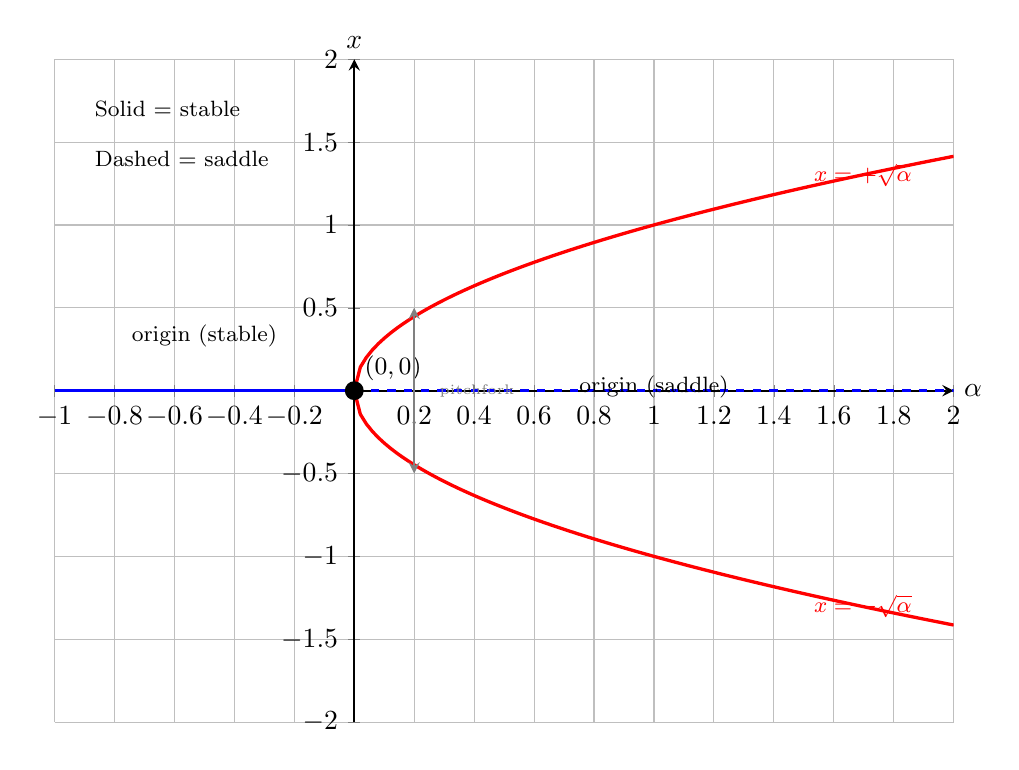
\begin{tikzpicture}
\begin{axis}[
    width=13cm,
    height=10cm,
    xlabel={$\alpha$},
    ylabel={$x$},
    xmin=-1, xmax=2,
    ymin=-2, ymax=2,
    grid=major,
    axis lines=middle,
    thick,
    every axis x label/.style={at={(current axis.right of origin)},anchor=west},
    every axis y label/.style={at={(current axis.above origin)},anchor=south}
]

% Branch 1: x = 0 stable (alpha < 0)
\addplot[blue, very thick, solid, domain=-1:0] {0};

% Branch 1: x = 0 unstable (alpha > 0)
\addplot[blue, very thick, dashed, domain=0:2] {0};

% Branch 2: x = sqrt(alpha) stable (alpha > 0)
\addplot[red, very thick, solid, domain=0:2, samples=100] {sqrt(x)};

% Branch 3: x = -sqrt(alpha) stable (alpha > 0)
\addplot[red, very thick, solid, domain=0:2, samples=100] {-sqrt(x)};

% Bifurcation point
\addplot[mark=*, mark size=3pt, black, only marks] coordinates {(0, 0)};
\node[above right, font=\small] at (axis cs:0,0) {$(0, 0)$};

% Labels
\node[anchor=south, font=\footnotesize] at (axis cs:-0.5,0.2) {origin (stable)};
\node[anchor=north, font=\footnotesize] at (axis cs:1,0.15) {origin (saddle)};
\node[red, anchor=west, font=\footnotesize] at (axis cs:1.5,1.3) {$x = +\sqrt{\alpha}$};
\node[red, anchor=west, font=\footnotesize] at (axis cs:1.5,-1.3) {$x = -\sqrt{\alpha}$};
\node[anchor=west, font=\footnotesize] at (axis cs:-0.9,1.7) {Solid = stable};
\node[anchor=west, font=\footnotesize] at (axis cs:-0.9,1.4) {Dashed = saddle};

% Pitchfork shape annotation
\draw[thick, <->, >=stealth, gray] (axis cs:0.2,0.5) -- (axis cs:0.2,0) -- (axis cs:0.2,-0.5);
\node[gray, font=\tiny, anchor=west] at (axis cs:0.25,0) {pitchfork};

\end{axis}
\end{tikzpicture}
\end{center}

\subsection*{XYZ Analysis of Bifurcation Diagram}

\begin{itemize}[leftmargin=*]
\item \stage{STAGE X (What the diagram shows):} One line for $\alpha < 0$ splitting into three lines for $\alpha > 0$, with the shape of a pitchfork. The middle prong (origin) changes from solid to dashed; the outer prongs are solid.

\item \stage{STAGE Y (Why this shape):} The curves $x = \pm\sqrt{\alpha}$ are parabolas on their side in $(\alpha, x)$ space:
\begin{itemize}
\item Squaring: $x^2 = \alpha$ describes a parabola opening to the right
\item This splits into two branches: $x = +\sqrt{\alpha}$ (upper) and $x = -\sqrt{\alpha}$ (lower)
\item Both branches meet at the origin when $\alpha = 0$ (vertex of parabola)
\item The square-root dependence $x \sim \sqrt{\alpha}$ means the branches grow slowly near $\alpha = 0$ - they emerge tangent to the horizontal line at $x = 0$
\end{itemize}
For $\alpha < 0$, only the origin branch exists (no real square roots of negative numbers). The pitchfork shape - one handle splitting into three prongs - gives the bifurcation its name.

\item \stage{STAGE Z (What this means dynamically):} Reading left to right as $\alpha$ increases:
\begin{itemize}
\item Far left ($\alpha \ll 0$): One stable equilibrium at origin; all trajectories attracted to $(0,0)$
\item Approaching zero: Still one attractor at origin
\item At zero: Critical point; one equilibrium with zero eigenvalue
\item Just past zero: Three equilibria appear; origin becomes saddle, two stable nodes emerge nearby
\item Far right ($\alpha \gg 0$): Two stable attractors at $x = \pm\sqrt{\alpha}$ far from origin; saddle at origin acts as separatrix
\end{itemize}
The system's attractor "bifurcates" - where there was one stable state, there are now two stable states symmetrically placed. This is spontaneous symmetry breaking: for $\alpha > 0$, the system must "choose" between $x > 0$ or $x < 0$ basins.
\end{itemize}

\vspace{10pt}
\hrule
\vspace{10pt}

\section{Step 8: Bifurcation Diagram ($\alpha$ vs $y$)}

\subsection*{Equilibrium curves in $(\alpha, y)$ space}

All equilibria have $y = 0$ (from $\dot{y} = -y = 0$).

Therefore, regardless of $\alpha$ or which equilibrium we consider:

\textbf{All branches:}
\[
y = 0 \quad \text{for all } \alpha
\]

\subsection*{Bifurcation diagram: $\alpha$ vs $y$}

\begin{center}
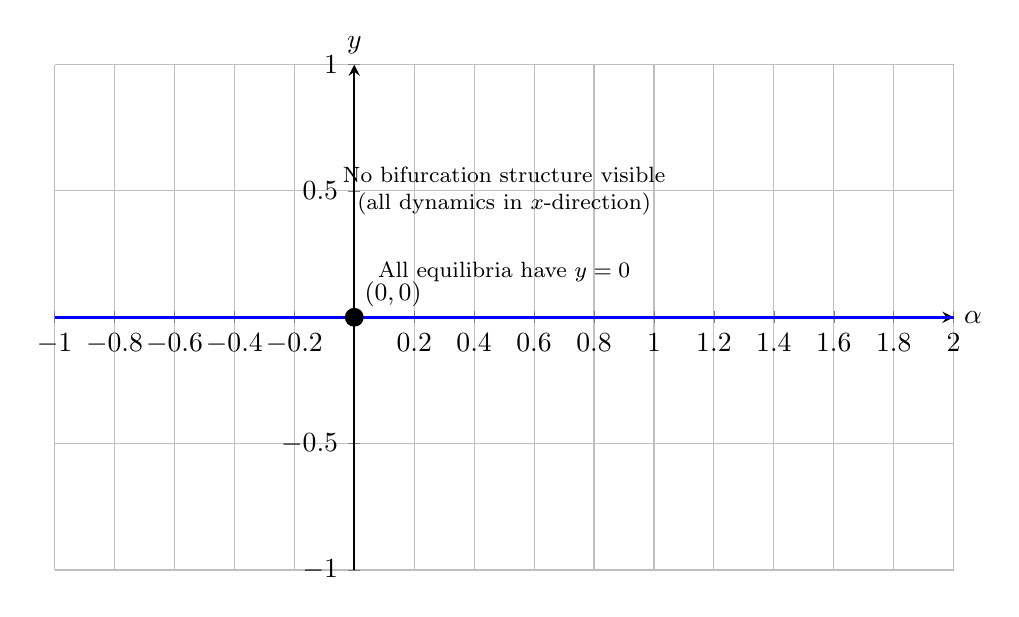
\begin{tikzpicture}
\begin{axis}[
    width=13cm,
    height=8cm,
    xlabel={$\alpha$},
    ylabel={$y$},
    xmin=-1, xmax=2,
    ymin=-1, ymax=1,
    grid=major,
    axis lines=middle,
    thick,
    every axis x label/.style={at={(current axis.right of origin)},anchor=west},
    every axis y label/.style={at={(current axis.above origin)},anchor=south}
]

% Single horizontal line at y = 0
\addplot[blue, very thick, solid, domain=-1:2] {0};

% Bifurcation point
\addplot[mark=*, mark size=3pt, black, only marks] coordinates {(0, 0)};
\node[above right, font=\small] at (axis cs:0,0) {$(0, 0)$};

% Label
\node[anchor=south, font=\footnotesize] at (axis cs:0.5,0.1) {All equilibria have $y = 0$};

% Note
\node[align=center, font=\footnotesize] at (axis cs:0.5,0.5) {No bifurcation structure visible \\ (all dynamics in $x$-direction)};

\end{axis}
\end{tikzpicture}
\end{center}

\subsection*{XYZ Analysis of $(\alpha, y)$ Diagram}

\begin{itemize}[leftmargin=*]
\item \stage{STAGE X (What we see):} A completely flat diagram - just a horizontal line at $y = 0$. No branches separate, no structure visible.

\item \stage{STAGE Y (Why this triviality):} The $y$-component of all equilibria is zero because:
\begin{itemize}
\item The equilibrium condition $\dot{y} = 0$ gives $-y = 0$, hence $y = 0$
\item This constraint is independent of $\alpha$ and independent of $x$
\item Whether we're at origin, $+\sqrt{\alpha}$, or $-\sqrt{\alpha}$, the $y$-coordinate is always zero
\item The decoupling means $y$-dynamics don't "know about" the bifurcation in $x$
\end{itemize}
In the $(\alpha, y)$ projection, all three equilibrium branches collapse onto the same line $y = 0$. We lose all information about the pitchfork structure because it occurs in the orthogonal ($x$) direction.

\item \stage{STAGE Z (What this reveals):} The bifurcation is fundamentally 1-dimensional - it happens in the $x$-direction. The $y$-direction is a "spectator":
\begin{itemize}
\item Always stable (exponential decay)
\item Always returns to $y = 0$
\item Doesn't participate in bifurcation
\end{itemize}
This demonstrates that bifurcation diagrams must be plotted against the relevant coordinate. Plotting against $y$ (the stable, non-bifurcating direction) reveals nothing. The choice of which coordinate to plot matters - we need the coordinate where the eigenvalue crosses zero.
\end{itemize}

\vspace{10pt}
\hrule
\vspace{10pt}

\section{Step 9: Phase Portraits}

\subsection*{Three scenarios}

\begin{center}
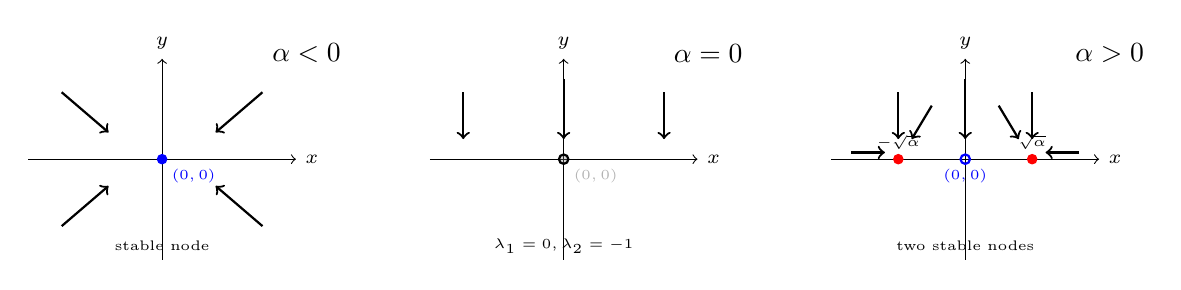
\begin{tikzpicture}[scale=0.85]
% alpha < 0
\begin{scope}
\draw[->] (-2,0) -- (2,0) node[right, font=\scriptsize] {$x$};
\draw[->] (0,-1.5) -- (0,1.5) node[above, font=\scriptsize] {$y$};
\node[above right] at (1.5,1.3) {$\alpha < 0$};
% Stable node at origin
\filldraw[blue] (0,0) circle (2pt) node[below right, font=\tiny] {$(0,0)$};
% Flows toward origin
\draw[->, thick] (-1.5,1) -- (-0.8,0.4);
\draw[->, thick] (1.5,1) -- (0.8,0.4);
\draw[->, thick] (-1.5,-1) -- (-0.8,-0.4);
\draw[->, thick] (1.5,-1) -- (0.8,-0.4);
\node[font=\tiny] at (0,-1.3) {stable node};
\end{scope}

% alpha = 0
\begin{scope}[shift={(6,0)}]
\draw[->] (-2,0) -- (2,0) node[right, font=\scriptsize] {$x$};
\draw[->] (0,-1.5) -- (0,1.5) node[above, font=\scriptsize] {$y$};
\node[above right] at (1.5,1.3) {$\alpha = 0$};
% Neutral equilibrium
\draw[black, thick, fill=gray, fill opacity=0.3] (0,0) circle (2pt) node[below right, font=\tiny] {$(0,0)$};
% Flows
\draw[->, thick] (-1.5,1) -- (-1.5,0.3);
\draw[->, thick] (1.5,1) -- (1.5,0.3);
\draw[->, thick] (0,1.2) -- (0,0.3);
\node[font=\tiny] at (0,-1.3) {$\lambda_1 = 0, \lambda_2 = -1$};
\end{scope}

% alpha > 0
\begin{scope}[shift={(12,0)}]
\draw[->] (-2,0) -- (2,0) node[right, font=\scriptsize] {$x$};
\draw[->] (0,-1.5) -- (0,1.5) node[above, font=\scriptsize] {$y$};
\node[above right] at (1.5,1.3) {$\alpha > 0$};
% Saddle at origin
\draw[blue, thick] (0,0) circle (2pt) node[below, font=\tiny] {$(0,0)$};
% Stable nodes at +/- sqrt(alpha)
\filldraw[red] (1,0) circle (2pt);
\node[font=\tiny, above] at (1,0) {$\sqrt{\alpha}$};
\filldraw[red] (-1,0) circle (2pt);
\node[font=\tiny, above] at (-1,0) {$-\sqrt{\alpha}$};
% Flows
\draw[->, thick] (1,1) -- (1,0.3);
\draw[->, thick] (-1,1) -- (-1,0.3);
\draw[->, thick] (0.5,0.8) -- (0.8,0.3);
\draw[->, thick] (-0.5,0.8) -- (-0.8,0.3);
\draw[->, thick] (0,1.2) -- (0,0.3);
\draw[->, thick] (-1.7,0.1) -- (-1.2,0.1);
\draw[->, thick] (1.7,0.1) -- (1.2,0.1);
\node[font=\tiny] at (0,-1.3) {two stable nodes};
\end{scope}
\end{tikzpicture}
\end{center}

\textit{Notation: Filled circle = stable, hollow circle = saddle}

\subsection*{XYZ Analysis of Phase Portrait Evolution}

\begin{itemize}[leftmargin=*]
\item \stage{STAGE X (What we see):} The single attractor at the origin splits into two symmetric attractors on the $x$-axis. All trajectories decay toward $y = 0$, then flow along the $x$-axis toward whichever stable equilibrium is nearest.

\item \stage{STAGE Y (Why these flows):} The decoupled structure creates two-stage dynamics:
\begin{itemize}
\item \textbf{Stage 1 (fast)}: $\dot{y} = -y$ causes rapid exponential decay toward $y = 0$. This happens on timescale $\tau \sim 1/|\lambda_2| = 1$.
\item \textbf{Stage 2 (slower near bifurcation)}: Once $y \approx 0$, motion is along $x$-axis governed by $\dot{x} = \alpha x - x^3$. Near the bifurcation ($\alpha \approx 0$), this is slow because the driving eigenvalue is small.
\end{itemize}

For $\alpha < 0$: The 1D flow $\dot{x} = \alpha x - x^3$ has $\dot{x} < 0$ for $x > 0$ (flow leftward) and $\dot{x} > 0$ for $x < 0$ (flow rightward), both toward origin.

For $\alpha > 0$: The 1D flow has three regions:
\begin{itemize}
\item $x < -\sqrt{\alpha}$: $\dot{x} < 0$ (flow left, away from basin)
\item $-\sqrt{\alpha} < x < 0$: $\dot{x} > 0$ (flow right, toward $-\sqrt{\alpha}$)
\item $0 < x < \sqrt{\alpha}$: $\dot{x} > 0$ (flow right, toward $\sqrt{\alpha}$)
\item $x > \sqrt{\alpha}$: $\dot{x} < 0$ (flow left, toward $\sqrt{\alpha}$)
\end{itemize}

\item \stage{STAGE Z (What this means globally):} Post-bifurcation, the phase plane splits into two basins of attraction:
\begin{itemize}
\item \textbf{Right basin} ($x > 0$): trajectories flow toward $(\sqrt{\alpha}, 0)$
\item \textbf{Left basin} ($x < 0$): trajectories flow toward $(-\sqrt{\alpha}, 0)$
\item \textbf{Separatrix}: the stable manifold of the saddle at origin (the $y$-axis) divides the basins
\end{itemize}
This is spontaneous symmetry breaking: the system is symmetric under $x \to -x$, but any trajectory starting away from $x = 0$ must "choose" one basin. The final state breaks the symmetry even though the equations preserve it. This phenomenon appears in physics (ferromagnets below Curie temperature), biology (left/right asymmetry in embryos), and many other contexts.
\end{itemize}

\vspace{10pt}
\hrule
\vspace{10pt}

\section{Summary}

\subsection*{Part (a): Equilibria and Stability}

\textbf{For all $\alpha$: all equilibria have $y = 0$ (from $\dot{y} = -y = 0$)}

\textbf{Equilibrium 1: $(0, 0)$}
\begin{itemize}
\item Always exists
\item Stable node for $\alpha < 0$ (eigenvalues: $\alpha < 0, -1$)
\item Neutral for $\alpha = 0$ (eigenvalues: $0, -1$)
\item Saddle for $\alpha > 0$ (eigenvalues: $\alpha > 0, -1$)
\end{itemize}

\textbf{Equilibria 2 and 3: $(\pm\sqrt{\alpha}, 0)$}
\begin{itemize}
\item Exist only for $\alpha > 0$
\item Both are stable nodes (eigenvalues: $-2\alpha < 0, -1$)
\item Emerge from origin at $\alpha = 0$
\item Move symmetrically along $x$-axis as $\pm\sqrt{\alpha}$
\end{itemize}

\subsection*{Part (b): Bifurcation at $\alpha = 0$}

\[
\boxed{\text{SUPERCRITICAL PITCHFORK BIFURCATION}}
\]

\textbf{Characteristics:}
\begin{itemize}
\item One equilibrium splits into three
\item System has reflectional symmetry: $f(-x) = -f(x)$
\item New equilibria are stable (supercritical)
\item Origin changes from stable node to saddle
\item One eigenvalue crosses zero
\end{itemize}

\subsection*{Part (c): Bifurcation Diagrams}

\textbf{$\alpha$ vs $x$ diagram:}
\begin{itemize}
\item Shows pitchfork structure
\item One branch ($x = 0$) for $\alpha < 0$ (solid)
\item Three branches for $\alpha > 0$:
  \begin{itemize}
  \item Center: $x = 0$ (dashed - saddle)
  \item Upper: $x = +\sqrt{\alpha}$ (solid - stable)
  \item Lower: $x = -\sqrt{\alpha}$ (solid - stable)
  \end{itemize}
\item Branches meet tangentially at $(\alpha, x) = (0, 0)$
\end{itemize}

\textbf{$\alpha$ vs $y$ diagram:}
\begin{itemize}
\item Completely trivial: $y = 0$ for all $\alpha$
\item No bifurcation structure visible
\item All equilibria collapse onto single horizontal line
\item Demonstrates bifurcation is 1D (in $x$-direction only)
\end{itemize}

\textbf{Key insight:} The bifurcation is confined to the $x$-direction where the eigenvalue crosses zero. The $y$-direction is always stable (spectator mode) and shows no bifurcation structure. Plotting against $y$ reveals nothing; plotting against $x$ reveals the pitchfork.

\end{document}
